\section{绘景}

\subsection{薛定谔绘景}

态矢量与实践有关, 算符(力学量)与时间无关, $t_0 \to t$,
态矢量随时间的演化由幺正算符$U(t, t_0) = e^{-\frac{i H
(t-t_0)}{\hbar}}$给出,

\begin{equation*}
\left| \Psi_S(t) \right\rangle = U(t, t_0) \left| \Psi_S(t_0)
\right\rangle
\end{equation*}

\subsection{相互作用绘景}

假设H不含时且可写为两项之和的形式,

\begin{equation*}
H = H_0 + H_1
\end{equation*}

定义相互作用绘景下态矢量,

\begin{equation*}
\left| \Psi_I (t) \right\rangle = e^{iH_0t/\hbar} \left|\Psi_S(t)
\right\rangle
\end{equation*}

$\left| \Psi_I (t) \right\rangle$满足,

\begin{equation*}
i \hbar \frac{\partial}{\partial t} \left| \Psi_I (t) \right\rangle
= H_1(t) \left| \Psi_I (t) \right\rangle
\end{equation*}

这里, $H_1(t)= e^{iH_0t/\hbar} H_1 e^{-iH_0t/\hbar}$,
在相互作用绘景下, 算符$O_I(t)$定义为:

\begin{equation*}
O_I(t)=e^{i H_0 t/\hbar} O_S e^{-i H_0 t/\hbar}
\end{equation*}

算符$O_I(t)$随时间的演化满足,

\begin{equation*}
i \hbar \frac{\partial}{\partial t} O_I (t) = \left[O_I(t), H_0
\right]
\end{equation*}

即$H_0$决定$O_I (t)$的演化, 而$H_1$决定$\left|\Psi_I(t)
\right\rangle$的演化。

\subsubsection{演化算符}

定义相互作用绘景下的演化算符, $U_I(t, t_0)$,

\begin{equation*}
\left| \Psi_I (t) \right\rangle = U_I (t, t_0)\left|\Psi_I (t_0)
\right\rangle
\end{equation*}

演化算符具有以下性质:

\begin{eqnarray*}
% \nonumber to remove numbering (before each equation)
  U_I (t_0, t_0) &=& 1 \\
  U_I^\dagger (t, t_0) U_I (t, t_0) &=& U_I (t, t_0) U_I^\dagger (t, t_0)
  = 1  \\
  U_I (t_1, t_2) U_I (t_2, t_3) &=& U_I (t_1, t_3) \\
  U_I (t, t_0) U_I (t_0, t) &=& 1
\end{eqnarray*}

$U_I$满足微分方程:

\begin{equation*}
i \hbar \frac{\partial }{\partial t} U_I (t, t_0) = H_1(t) U_I(t,
t_0)
\end{equation*}

形式解为(以下$U_I$简记为$U$):

\begin{equation*}
U(t, t_0) = 1- \frac{i}{\hbar}\int_{t_0}^t dt' H_1(t') U(t', t_0)
\end{equation*}

由此可得到迭代解,

\begin{equation*}
U(t, t_0) = \sum_{n=0}^{\infty} \left( \frac{-i}{\hbar} \right)^n
\frac{1}{n!}\int_{t_0}^t ... \int_{t_0}^t dt_1 ... dt_n T \left[
H_1(t_1)...H_1(t_n) \right]
\end{equation*}

很重要地, 这里引入了编时算符$T$,
以保证“被积函数”中的算符对易关系不被破坏。编时算符的作用是使算符按从早到晚的次序, 自右向左排列。

\subsection{海森堡绘景}

态矢量定义为,

\begin{equation*}
\left| \Psi_H (t) \right\rangle = e^{iHt / \hbar} \left| \Psi_S(t)
\right\rangle
\end{equation*}

不随时间演化. 可记为$\left| \Psi_H \right\rangle$.

力学量,

\begin{equation*}
O_H (t) = e^{i Ht / \hbar} O_S e^{-i Ht / \hbar}
\end{equation*}

随时间演化。满足海森堡运动方程,

\begin{equation*}
i \hbar \frac{\partial }{\partial t} O_H (t) = \left[ O_H (t), H
\right]
\end{equation*}

小结一下的话:

\begin{eqnarray*}
% \nonumber to remove numbering (before each equation)
  \left| \Psi_H \right\rangle &=& \left| \Psi_S (0) \right\rangle =  \left| \Psi_I (0) \right\rangle\\
  O_S &=& O_H (0) = O_I (0)
\end{eqnarray*}

\subsection{绝热假设}

要计算传播子(\ref{1 quasiparticle propagation}),
我们需要构造如下“绝热过程”:

\begin{figure}[h]
\begin{center}
  % Requires \usepackage{graphicx}
  \includegraphics[width=8cm]{Zero/juerejinsi.ps}\\
%  \caption{}\label{}
\end{center}
\end{figure}

在$t \to - \infty$时, 粒子间无相互作用, $H = H_0$, 态矢量为,

\begin{equation*}
\left| \Psi_I (t \to - \infty) \right\rangle = \left| \Phi_0
\right\rangle
\end{equation*}

$t= - \infty \to t=0$, 逐渐引入相互作用, 此时达到真正的基态。

\begin{equation*}
\left|\Psi_H^0 \right\rangle = U(0, -\infty) \left| \Psi_I(-\infty)
\right\rangle =  U(0, -\infty) \left| \Phi_0 \right\rangle
\end{equation*}


$t=0 \to t = \infty$, 再逐渐去掉相互作用,

\begin{equation*}
U(\infty,0) \left|\Psi_H^0 \right\rangle =
U(\infty,-\infty)\left|\Phi_0 \right\rangle = S\left|\Phi_0
\right\rangle
\end{equation*}

这里的$S = U(\infty, -\infty)$,
叫做S矩阵。在经历了绝热加场和绝热去场后, $S \left|
\right\rangle$仍然是$H_0$的基态, 最多可能相差一个相位因子$e^{-iL}$,
即:


\begin{equation}\label{S matrix}
S \left| \Phi_0 \right\rangle = e^{-iL} \left| \Phi_0 \right\rangle
\end{equation}

因此,

\begin{equation*}
\left| \Psi_H^0 \right\rangle = U(0, \infty) U(\infty, -\infty)
\left| \Phi_0 \right\rangle = U(0, \infty) \left| \Phi_0
\right\rangle e^{-iL}
\end{equation*}

此时, 我们已经用已知的“无相互基态”$\left| \Phi_0
\right\rangle$表示了我们真正感兴趣的“相互作用基态”$\left| \Psi_H^0
\right\rangle$.

现在我们来计算“几率幅”,

\begin{equation}\label{TAHBH}
\left\langle \Psi_H^0 \right| T \left( A_H(t_1) B_H(t_2) \right)
\left| \Psi_H^0 \right\rangle
\end{equation}

上式实际上就是我们关心的“传播子”(\ref{1 quasiparticle
propagation}), 只是写法上更具一般性。我们可以把$\left| \Psi_H^0 \right\rangle = U(0, \infty) \left| \Phi_0 \right\rangle
e^{-iL}$代入上式中, 并化简, 可得:


\begin{equation*}
e^{iL} \left\langle \Phi_0 \right| U(\infty, 0) T \left( A_H (t_1)
B_H(t_2) \right) U(0, -\infty) \left| \Phi_0 \right\rangle
\end{equation*}


可以证明相互作用绘景和海森堡绘景之间的联系是:

\begin{equation*}
O_H(t) = U(0,t)O_I(t) U(t,0)
\end{equation*}


利用上式, 我们可把公式(\ref{TAHBH})化简为:

\begin{equation}\label{TABHeiL}
e^{iL} \left\langle \Phi_0 \right| T \left( A_I(t_1) B_I(t_2) S
\right) \left| \Phi_0 \right\rangle
\end{equation}


由S矩阵(\ref{S matrix}), 我们可得相位因子$e^{iL}$的表达式,

\begin{equation*}
e^{iL} = \frac{1}{\left\langle \Phi_0 \right|S \left| \Phi_0
\right\rangle}
\end{equation*}

将其代入公式(\ref{TABHeiL}), 最终我们得到:

\begin{equation}\label{TABoverPhiSquared}
\left\langle \Psi_H^0 \right| T \left( A_H(t_1) B_H(t_2) \right)
\left| \Psi_H^0 \right\rangle = \frac{\left\langle \Phi_0 \right| T
\left( A_I(t_1) B_I(t_2) S \right) \left| \Phi_0
\right\rangle}{\left\langle \Phi_0 \right| S \left| \Phi_0
\right\rangle}
\end{equation}

关于绝热假设的正确性, 需要用到盖尔曼和罗定理(Gell-Mann and Low Theorem\footnote{M. Gell-Mann and F. Low, \textit{Phys. Rev.},
\textbf{84}: 350 (1951).}), 盖尔曼和罗证明: 在从$t \to -
\infty$无限缓慢地引入相互作用后, 从“无相互作用基态”$\left| \Phi_0 \right\rangle$出发所达到的态(在$t=0$时)是H的本征态, 但不一定是系统的基态。

所以, 只有当在引入相互作用后, 基态能量只发生移动,
而不发生能谱结构的重新变化, 如“粒子的产生、湮灭算符重组”后出现新的更低能量的态(超导的BCS凝聚), 则绝热假设成立。关于绝热假设, 更多请阅读费特和瓦立克书pp72.


\subsection*{练习}

证明相互作用绘景和海森堡绘景之间的联系是:

\begin{equation*}
O_H(t) = U(0,t)O_I(t) U(t,0)
\end{equation*}

这里$O_H(t)$是海森堡绘景下算符, $O_I (t)$是相互作用绘景下算符,
$U$是相互作用绘景下的演化算符。

证:

根据海森堡绘景和相互作用绘景的定义,

\begin{eqnarray*}
% \nonumber to remove numbering (before each equation)
  O_H(t) &=& e^{iHt/ \hbar}O_S e^{-iHt/ \hbar} \\
  O_I(t) &=& e^{iH_0t/ \hbar}O_S e^{-iH_0t/ \hbar}
\end{eqnarray*}

力学量的期望值$\left\langle O \right\rangle $,

\begin{eqnarray*}
% \nonumber to remove numbering (before each equation)
  \left\langle O \right\rangle &=& \left\langle \psi_S(t)\right| O_S \left| \psi_S(t) \right\rangle = \left\langle \psi_H \right| O_H(t) \left| \psi_H \right\rangle\\
  {} &=& \left\langle \psi_H \right|  e^{iHt/ \hbar} O_S e^{-iHt/ \hbar}  \left| \psi_H
  \right\rangle \\
  {} &=& \left\langle \psi_S(t)\right|  e^{-iH_0t/ \hbar} e^{iH_0t/ \hbar} O_S e^{-iH_0t/ \hbar} e^{iH_0t/ \hbar} \left| \psi_S(t)
  \right\rangle \\
  {} &=& ... O_I(t) e^{i H_0 t/ \hbar} e^{-i Ht/ \hbar} e^{i Ht/
  \hbar} \left| \psi_S(t) \right\rangle
\end{eqnarray*}


$t=0$时, 三种绘景重合, 此时有:

\begin{equation*}
\left| \psi_H \right\rangle = \left|\psi_S(t=0) \right\rangle =
e^{iHt/ \hbar} \left| \psi_S(t) \right\rangle
\end{equation*}

因此,

\begin{equation*}
    O_H (t) = e^{iHt/\hbar} e^{-iH_0t/\hbar} O_I(t) e^{iH_0t/\hbar} e^{-iHt/\hbar}
\end{equation*}

考虑到,

\begin{eqnarray*}
% \nonumber to remove numbering (before each equation)
\left| \psi_I(t) \right\rangle &=& e^{i H_0 t/ \hbar} \left|
\psi_S(t)\right\rangle \\
  {} &=& e^{i H_0 t/ \hbar} e^{-iHt/\hbar} \left|
\psi_S(0) \right\rangle \\
  {} &=& e^{i H_0 t/ \hbar} e^{-iHt/\hbar} \left|
\psi_I(0) \right\rangle
\end{eqnarray*}

因此,

\begin{equation*}
    U_I (t) = e^{iH_0t/\hbar}e^{-iHt/\hbar}
\end{equation*}

因此,

\begin{equation*}
O_H (t) = U_I(-t)O_I(t)U_I(t)
\end{equation*}

QED

\subsection*{阅读}

\begin{enumerate}

  \item 费特, 瓦立克, 《多粒子系统的量子理论》, $\S$ 3.6.

  \item 蔡建华 等, 《量子统计的格林函数理论》, $\S$ 2.1.

  \item G. D. Mahan, Many-Particle Physics, $\S$ 2.1-2.

\end{enumerate}